  \let\negmedspace\undefined
\let\negthickspace\undefined
\documentclass[journal]{IEEEtran}
\usepackage[a5paper, margin=10mm, onecolumn]{geometry}
\usepackage{lmodern} % Ensure lmodern is loaded for pdflatex
\usepackage{tfrupee} % Include tfrupee package

\setlength{\headheight}{1cm} % Set the height of the header box
\setlength{\headsep}{0mm}     % Set the distance between the header box and the top of the text

\usepackage{gvv-book}
\usepackage{gvv}
\usepackage{cite}
\usepackage{amsmath,amssymb,amsfonts,amsthm}
\usepackage{algorithmic}
\usepackage{graphicx}
\usepackage{textcomp}
\usepackage{xcolor}
\usepackage{txfonts}
\usepackage{listings}
\usepackage{enumitem}
\usepackage{mathtools}
\usepackage{gensymb}
\usepackage{comment}
\usepackage[breaklinks=true]{hyperref}
\usepackage{tkz-euclide} 
\usepackage{listings}                                      
\def\inputGnumericTable{}                                 
\usepackage[latin1]{inputenc}                                
\usepackage{color}                                            
\usepackage{array}                                            
\usepackage{longtable}
\usepackage{multicol}
\usepackage{calc}                                             
\usepackage{multirow}                                         
\usepackage{hhline}                                           
\usepackage{ifthen}                                           
\usepackage{lscape}
\begin{document}
	
	\bibliographystyle{IEEEtran}
	\vspace{3cm}
	
	\title{9.ex.24}
	\author{EE24BTECH11059 - Y Siddhanth}
	% \maketitle
	% \newpage
	% \bigskip
	{\let\newpage\relax\maketitle}
	
	\renewcommand{\thefigure}{\theenumi}
	\renewcommand{\thetable}{\theenumi}
	\setlength{\intextsep}{10pt} % Space between text and floats
	
	
	\numberwithin{equation}{enumi}
	\numberwithin{figure}{enumi}
	\renewcommand{\thetable}{\theenumi}
	
	
	\textbf{Question}:\newline
	Find the solution of the given differential equation$$\frac{d^2y}{dx^2} - 2a \frac{dy}{dx} + (a^2 + b^2)y = 0 $$. \\
	\textbf{Solution: }\\
	Theoretical Solution: \\
	To apply $\mathcal{L}$-Transform to the above equation, we define:
	\begin{align}
		\mathcal{L}\left\{\frac{d^2y}{dx^2}\right\} &= s^2 Y(s) - s y(0) - y'(0) \\
		\mathcal{L}\left\{\frac{dy}{dx}\right\} &= s Y(s) - y(0) \\
		\mathcal{L}\{y(x)\} &= Y(s)
	\end{align}
	Taking the $\mathcal{L}$-Transform of the equation:
	\begin{align}
		\mathcal{L}\left\{\frac{d^2y}{dx^2}\right\} - 2a \mathcal{L}\left\{\frac{dy}{dx}\right\} + (a^2 + b^2) \mathcal{L}\{y\} = 0 \\
		\big(s^2 Y(s) - s y(0) - y'(0)\big) - 2a \big(s Y(s) - y(0)\big) + (a^2 + b^2) Y(s) = 0 \\
		\big(s^2 - 2as + (a^2 + b^2)\big) Y(s) = \big(s y(0) + y'(0)\big) - 2a y(0))
	\end{align}
	Thus, $Y(s)$ can be written as, 
	\begin{align}
	 	Y(s) &= \frac{\big(s y(0) + y'(0)\big) - 2a y(0))}{	\big(s^2 - 2as + (a^2 + b^2)\big)}\\
	\end{align}
	We get, 
	\begin{align}
		Y(s) &= \frac{s y(0) + y'(0) - 2a y(0)}{(s - a)^2 + b^2}\\
	\end{align}
	To apply partial fractions, we can rewrite the above as:
	\begin{align}
				Y(s) &= \frac{A(s - a) + B}{(s - a)^2 + b^2} \label{Y}
	\end{align}
	Using the inverse Laplace transform formulas:
	\begin{align}
		\mathcal{L}^{-1}\left\{\frac{s - a}{(s - a)^2 + b^2}\right\} &= e^{ax} \cos(bx)u(x), \\
		\mathcal{L}^{-1}\left\{\frac{1}{(s - a)^2 + b^2}\right\} &= \frac{1}{b} e^{ax} \sin(bx)u(x),
	\end{align}
	Thus, general solution is then:
	\begin{align}
		y(x) &= e^{ax} \big(C_1 \cos(bx) + C_2 \sin(bx)\big)u(x),
	\end{align}
	Taking initial conditions as $(0,1)$, $\frac{dy}{dx} = 1$ and $a=1,b=1$, we get
		\begin{align}
					y(x) &= e^{x}\cos(x)u(x)
		\end{align}
	\newline
	Numerical Solution:\newline
	We have to apply the trapezoidal rule,
	\begin{align}
		J &= \int_a^b f\brak{x}\, dx\\
		&\approx h\brak{\frac{1}{2}f\brak{a} + f\brak{x_1} + f\brak{x_2} \cdots + f\brak{x_{n-1}} + \frac{1}{2}f\brak{b}}\\
	\end{align}
	Discretizing the steps using trapezoidal rule for $y^{\prime\prime}  = f(x,y,y^\prime) = 2y^\prime - 2y$ gives us
	\begin{align}
		y^\prime_{n+1}  &= y^\prime_n + \frac{h}{2}\brak{f(x_n,y_n,y_n^\prime) + f(x_{n+1},y_{n+1},y_{n+1}^\prime)} \\
		y^\prime_{n+1}  &= y^\prime_n + \frac{h}{2}\brak{ 2y^\prime_{n+1} - 2y_{n+1} + 2y^\prime_{n} - 2y_{n}} \label{1}\\
		y_{n+1}  &= y_n + \frac{h}{2}\brak{y^\prime_{n+1} + y^\prime_n} \label{2}\\
	\end{align}
	Solving \eqref{1}, \eqref{2},
	\begin{align}
		y^\prime_{n+1}  &= y^\prime_n\brak{\frac{1+ h - \frac{h^2}{2}}{1- h + \frac{h^2}{2}}} - \brak{\frac{2h}{1- h + \frac{h^2}{2}}}y_n\\
		y_{n+1}  &= y_n + \frac{h}{2}\brak{y^\prime_n\brak{\frac{1+ h - \frac{h^2}{2}}{1- h + \frac{h^2}{2}}} - \brak{\frac{2h}{1- h + \frac{h^2}{2}}}y_n + y^\prime_n} \label{2}\\
	\end{align}
	By applying the above 2 equations iteratively, we can plot the curve. \\
	Alternatively, we can using the bilinear transform on \eqref{Y} to find a more accurate difference equation.
	\begin{align}
		s &= \frac{2}{h} \frac{1-z^{-1}}{1+z^{-1}}\\
		Y(s) &= \frac{s - 1}{(s -1)^2 + 1} \\
		Y(z) &= \frac{\frac{2}{h} \frac{1-z^{-1}}{1+z^{-1}} - 1}{(\frac{2}{h} \frac{1-z^{-1}}{1+z^{-1}} -1)^2 + 1} \\
	\end{align}
	Simplifying it,we get:
		\begin{align}
		Y(z) &= \frac{2\brak{\brak{h - \frac{h^2}{2}} - h^2 z^{-1} + \brak{-h - \frac{h^2}{2}}z^{-2}}}{\brak{  \brak{2-h}^2 + h^2} + 2z^{-1}\brak{2h^2 - 4} + \brak{  \brak{2+h}^2 + h^2}z^{-2} }\end{align}
		\begin{align}
		{\brak{  \brak{2-h}^2 + h^2}Y(z)  + 2z^{-1}Y(z) \brak{2h^2 - 4} + \brak{  \brak{2+h}^2 + h^2}z^{-2} }Y(z)\\
		=  {2\brak{\brak{h - \frac{h^2}{2}} - h^2 z^{-1} + \brak{-h - \frac{h^2}{2}}z^{-2}}}
	\end{align}
	Applying inverse-$Z$ transform, we get
	\begin{align}
		\quad y_n = -2y_{n-1} \cdot \frac{2h^2 - 4}{(2-h)^2 + h^2} - y_{n-2}\cdot \frac{(2+h)^2 + h^2}{(2-h)^2 + h^2} \\ 
		+ \frac{2\brak{\brak{h- \frac{h^2}{2}}\delta[n]  - h^2 \delta[n-1] + \brak{-h - \frac{h^2}{2}}\delta[n-2]}}{(2-h)^2 + h^2}
	\end{align}
	Plotting Bilinear Transform(Sim2) and Trapezoidal Rule(Sim1), we get
	\begin{figure}[h!]
		\centering
		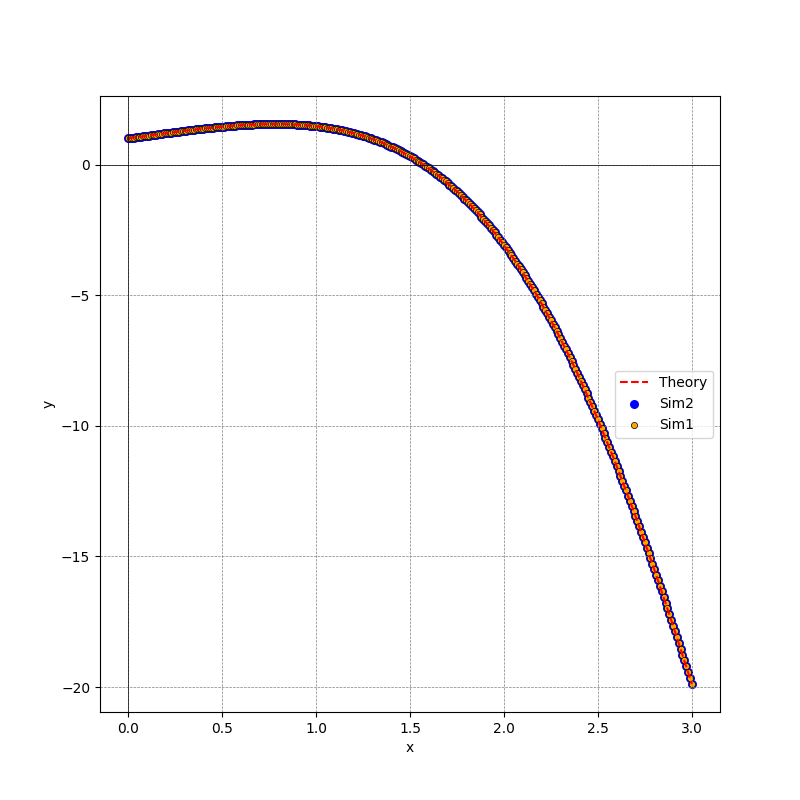
\includegraphics[width=\columnwidth]{figs/fig1.png}
		\caption{Comparison between the Theoretical solution and Numerical solution}
		\label{stemplot}
	\end{figure}
	
\end{document}  